\section{Suddivisione del lavoro}
I componenti del gruppo dovranno rivestire ciascuno, almeno una volta, tutti i ruoli specificati nel \textit{organigramma}.
Durante le varie fasi ogni componente può ricoprire più ruoli, anche contemporaneamente, purchè non si presentino dei conflitti di interesse tra le attività svolte. Ad esempio un componente non può essere verificatore di se stesso.
\subsection{Analisi dei Requisiti}
Nell'attività di \textbf{Analisi}, ciascun componente dovrà rivestire i seguenti ruoli:
\begin{table}[H]
	\begin{center}
		\begin{tabular}{|c|c|c|c|c|c|c|c|}
			\hline
			\textbf{Nominativo} & \multicolumn{6}{c|}{\textbf{Ore per ruolo}} & \textbf{Ore totali} \\
			& \textbf{Re} & \textbf{Am} & \textbf{An} & \textbf{Pj} & \textbf{Pr} & \textbf{Ve} & \\
			\hline
			Berton Franco		&		&	4	&	26	&		&		&		&	30	\\
			\hline
			Ferrara Alberto		&		&	6	&	24	&	 	&		&		& 	30	\\
			\hline
			Gnoato Matteo		&	21	&		&	9	&		&		&		&	30	\\
			\hline						
			Granzotto Matteo	&	22	&	 	&	8 	&		&	 	& 		&	30	\\
			\hline
			Magagna Simone 		&		&	4	&	5	&		&		& 	21	&	30	\\
			\hline
			Prelaz Marco 		& 		&		&	7	&		&		&	23	&	30	\\
			\hline						
			Varotto Mattia 		&		&	4	&	5	&		&		&	21	& 	30	\\
			\hline
		\end{tabular}
	\end{center}
	\caption{Ore per componente, Analisi dei Requisiti}
\end{table}

\begin{figure}[H]
	\centering
	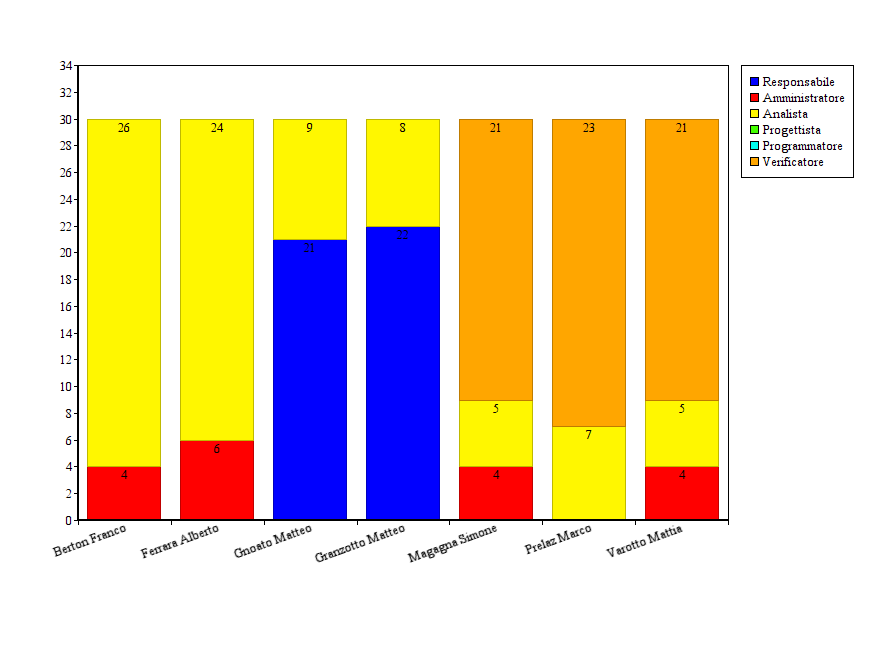
\includegraphics[scale=0.4]{immagini/Grafi/GrafoAR}
	\caption{Incidenza ore per ruolo, Analisi dei Requisiti}
\end{figure}

\subsection{Progettazione Architetturale}
Nel periodo di \textbf{Progettazione Architetturale} ciascun componente del gruppo dovrà rivestire i seguenti ruoli:
\begin{table}[H]
	\begin{center}
		\begin{tabular}{|c|c|c|c|c|c|c|c|}
			\hline
			\textbf{Nominativo} & \multicolumn{6}{c|}{\textbf{Ore per ruolo}} & \textbf{Ore totali} \\
			& \textbf{Re} & \textbf{Am} & \textbf{An} & \textbf{Pj} & \textbf{Pr} & \textbf{Ve} & \\
			\hline
			Berton Franco		&		&		&		&	10	&		&	23	&	33	\\
			\hline
			Ferrara Alberto		&		&		&		&	9 	&		&	23	& 	32	\\
			\hline
			Gnoato Matteo		&		&		&		&	8	&		&	24	&	32	\\
			\hline									
			Granzotto Matteo	&		&	 4	&  		&	28	&	 	& 		&	32	\\
			\hline
			Magagna Simone 		&	3	&		&		&	29	&		& 		&	32	\\
			\hline
			Prelaz Marco 		& 		&	4	&		&	28	&		&		&	32	\\
			\hline						
			Varotto Mattia 		&	3	&		&		&	29	&		&		& 	32	\\
			\hline
		\end{tabular}
	\end{center}
	\caption{Ore per componente, Progettazione Architetturale}
\end{table}

\begin{figure}[H]
	\centering
	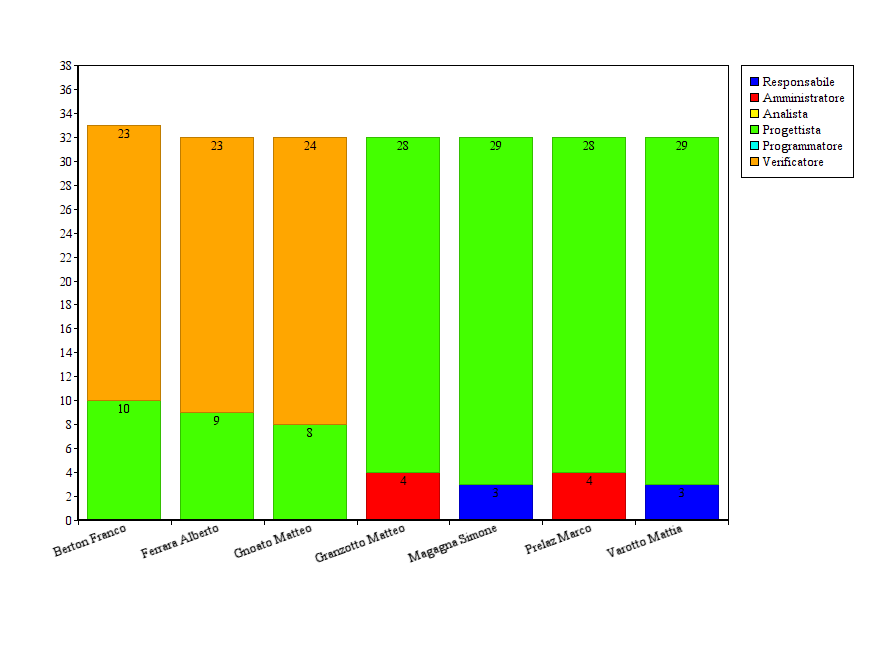
\includegraphics[scale=0.4]{immagini/Grafi/GrafoPA}
	\caption{Incidenza ore per ruolo, Progettazione Architetturale}
\end{figure}

\subsection{Progettazione di Dettaglio}
Nel periodo di \textbf{Progettazione di Dettaglio} ciascun componente del gruppo dovrà rivestire i seguenti ruoli:
\begin{table}[H]
	\begin{center}
		\begin{tabular}{|c|c|c|c|c|c|c|c|}
			\hline
			\textbf{Nominativo} & \multicolumn{6}{c|}{\textbf{Ore per ruolo}} & \textbf{Ore totali} \\
			& \textbf{Re} & \textbf{Am} & \textbf{An} & \textbf{Pj} & \textbf{Pr} & \textbf{Ve} & \\
			\hline
			Berton Franco		&	3	&		&		&	17	&		&		&	20	\\ 
			\hline
			Ferrara Alberto		&	4	&		&		&	16	&		&		& 	20	\\ 
			\hline
			Gnoato Matteo		&		&	2	&		&	18	&		&		&	20	\\ 
			\hline									
			Granzotto Matteo	&		&	 	&		&	6	&	 	& 	14	&	20	\\
			\hline
			Magagna Simone 		&		&	3	&		&	17	&		& 		&	20	\\ 
			\hline
			Prelaz Marco 		& 		&		&		&	6	&		&	14	&	20	\\ 
			\hline
			Varotto Mattia 		&		&		&		&	6	&		&	14	& 	20	\\ 
			\hline
		\end{tabular}
	\end{center}
	\caption{Ore per componente,Progettazione di Dettaglio}
\end{table}

\begin{figure}[H]
	\centering
	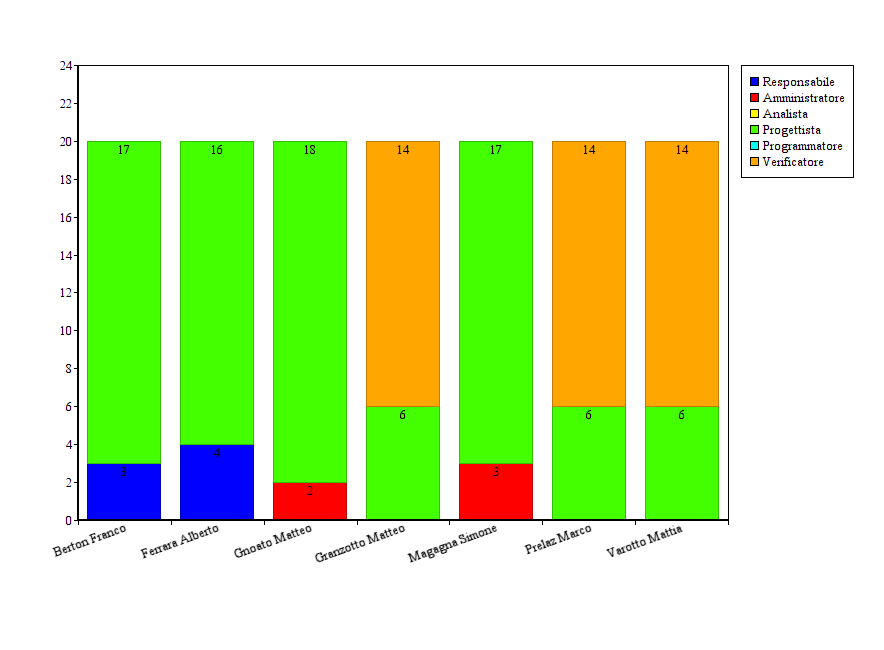
\includegraphics[scale=0.4]{immagini/Grafi/GrafoPD}
	\caption{Incidenza ore per ruolo, Progettazione di Dettaglio}
\end{figure}

\subsection{Codifica}
Nel periodo di \textbf{Codifica} ciascun componente del gruppo dovrà rivestire i seguenti ruoli:
\begin{table}[H]
	\begin{center}
		\begin{tabular}{|c|c|c|c|c|c|c|c|}
			\hline
			\textbf{Nominativo} & \multicolumn{6}{c|}{\textbf{Ore per ruolo}} & \textbf{Ore totali} \\
			& \textbf{Re} & \textbf{Am} & \textbf{An} & \textbf{Pj} & \textbf{Pr} & \textbf{Ve} & \\
			\hline
			Berton Franco		&		&		&		&		&	35	&		&	35	\\
			\hline	
			Ferrara Alberto		&		&		&		&	 5	&	31	&		& 	36	\\
			\hline		
			Gnoato Matteo		&		&	4	&		&		&	7	&	25	&	36	\\
			\hline						
			Granzotto Matteo	&	5	&	 	&		&	5	&	25 	& 		&	35	\\
			\hline
			Magagna Simone 		&		&		&		&	5	&	5	& 	25	&	35	\\
			\hline
			Prelaz Marco 		& 	6	&		&		&	5	&	24	&		&	35	\\
			\hline
			Varotto Mattia 		&		&		&		&	5	&	6	&	25	& 	36	\\
			\hline			
		\end{tabular}
	\end{center}
	\caption{Ore per componente, Analisi dei Requisiti}
\end{table}

\begin{figure}[H]
	\centering
	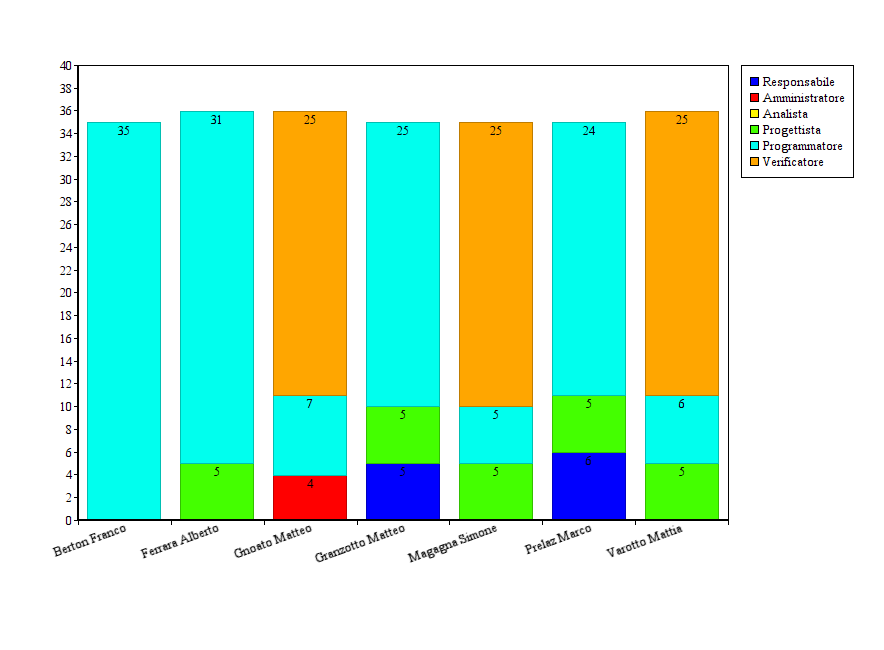
\includegraphics[scale=0.4]{immagini/Grafi/GrafoCod}
	\caption{Incidenza ore per ruolo, Codifica}
\end{figure}

\subsection{Verifica e Validazione}
Nel periodo di \textbf{Verifica e Validazione} ciascun componente del gruppo dovrà rivestire i seguenti ruoli:
\begin{table}[H]
	\begin{center}
		\begin{tabular}{|c|c|c|c|c|c|c|c|}
			\hline
			\textbf{Nominativo} & \multicolumn{6}{c|}{\textbf{Ore per ruolo}} & \textbf{Ore totali} \\
			& \textbf{Re} & \textbf{Am} & \textbf{An} & \textbf{Pj} & \textbf{Pr} & \textbf{Ve} & \\
			\hline
			Berton Franco		&		&		&		&	6	&		&	11	&	17	\\
			\hline
			Ferrara Alberto		&		&		&		&	 6	&		&	11	& 	17	\\
			\hline	
			Gnoato Matteo		&		&		&		&	8	&		&	9	&	17	\\
			\hline								
			Granzotto Matteo	&		&	 	&		&		&	 	& 	18	&	18	\\
			\hline
			Magagna Simone 		&	9	&		&		&		&		& 	9	&	18	\\
			\hline	
			Prelaz Marco 		& 		&		&		&		&		&	18	&	17	\\
			\hline					
			Varotto Mattia 		&		&		&		&		&		&	17	& 	17	\\
			\hline
		\end{tabular}
	\end{center}
	\caption{Ore per componente, Verifica e Validazione}
\end{table}

\begin{figure}[H]
	\centering
	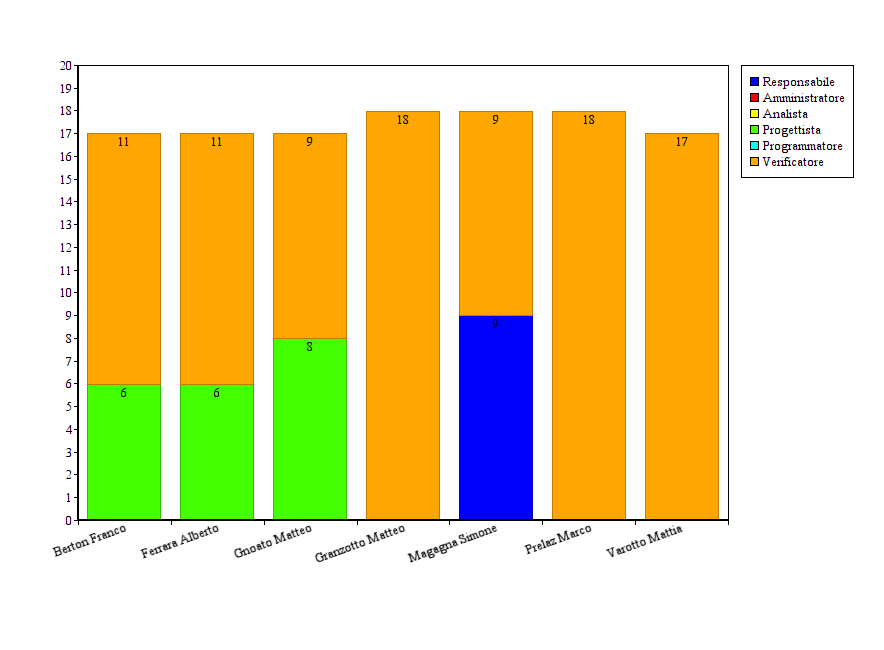
\includegraphics[scale=0.4]{immagini/Grafi/GrafoVV}
	\caption{Incidenza ore per ruolo, Verifica e Validazione}
\end{figure}

\subsection{Totali}
La tabella seguente illustra le ore totali che ogni componente dedicherà per il progetto, mettendo in evidenza anche quelle che verrano poi redicontate.
\begin{table}[H]
	\begin{center}
		\begin{tabular}{|c|c|c|c|c|c|c|c|c|}
			\hline
			\multirow{2}{*}{\textbf{Nominativo}} & & \multicolumn{6}{c|}{\textbf{Ore per ruolo}} & \multirow{2}{*}{\textbf{Ore totali}} \\
			& & \textbf{Re} & \textbf{Am} & \textbf{An} & \textbf{Pj} & \textbf{Pr} & \textbf{Ve} & \\
			\hline
			\hline
			\multirow{2}{*}{Berton Franco}		&	Rendicontate	&	3	&	0	&	0	&	33	&	35	& 34 	&	105	\\
			\cline{2-9}
			&	Totali			&	3	&	4	&	26	&	33	&	35	& 	34	&	135	\\
			\hline	
			\hline
			\multirow{2}{*}{Ferrara Alberto}	&	Rendicontate	&	4	&	0	&	0	&	35	&	31	&  34	&	105	\\
			\cline{2-9}
			&	Totali			&	4	&	6	&	24	&	35	&	31	& 	34	&	135	\\
			\hline
			\hline
			\multirow{2}{*}{Gnoato Matteo}	&	Rendicontate	&	0	&	6	&	0	&	34	&	7	&	58	&	105	\\
			\cline{2-9}
			&	Totali			&	21	&	6	&	9	&	34	&	7	&	58	&	135	\\
			\hline
			\hline					
			\multirow{2}{*}{Granzotto Matteo}	&	Rendicontate	&	5	&	4	&	0	&	39	&	25	&	32	&	105	\\
			\cline{2-9}
			&	Totali			&	27	&	4	&	8	&	39	&	25	&	32	&	135	\\
			\hline
			\hline
			\multirow{2}{*}{Magagna Simone}		&	Rendicontate	&	12	&	3	&	0	&	51	&	5	& 	34	&	105	\\
			\cline{2-9}
			&	Totali			&	12	&	7	&	5	&	51	&	5	& 	55	&	135	\\
			\hline			
			\hline
			\multirow{2}{*}{Prelaz Marco}	&	Rendicontate	&	6	&	4	&	0	&	39	&	24	& 	32	&	105	\\
			\cline{2-9}
			&	Totali			&	6	&	4	&	7	&	39	&	24	& 	55	&	135	\\
			\hline
			\hline			
			\multirow{2}{*}{Varotto Mattia}	&	Rendicontate	&	3	&	0	&	0	&	40	&	6	& 	56	&	105	\\
			\cline{2-9}
			&	Totali			&	3	&	4	&	5	&	40	&	6	& 	77	&	135	\\
			\hline
		\end{tabular}
	\end{center}
	\caption{Ore per componente per ruolo, rendicontate e totali}
\end{table}
